\section{Introduction}\label{intro}
Optimization problems are problems in which the goal is to locate a set of inputs $x \in \mathbb{R}^{n}$ that result in the minima or maxima of a target objective function. In this thesis the problem of minimizing an objective function often called a cost function will be considered. Such an optimization problem takes the form:
\begin{equation*}\label{eq:1}\tag{2.1}
\begin{aligned}
    &\text{minimize} \ f_{0}(x) \\
    &\text{subject to} \ f_{i}(x) \leq b_{i}, \text{  } i=1,\ldots,m 
\end{aligned}
\end{equation*}
Here the vector $x=(x_{1},\ldots,x_{n})$ is called the optimization variable, the function $f_{0}: \mathbb{R}^{n} \longrightarrow \mathbb{R}$ is the objective function, the functions $f_{i}: \mathbb{R}^{n} \longrightarrow \mathbb{R}, \text{  }i=1,\ldots,m$ are the constraint functions and the constants $b_{1},\ldots,b_{m}$ are the bounds for the constraints. A vector $x^{*}$ is called an optimal solution to the problem if the function $f_{0}$ attains either a local or a global minimum at $x^{*}$. The concepts of a local minimum and a global minimum are formally defined as follows:
\begin{definition}(\cite[235]{adams2013calculus})\label{local_min}
We say that a function $f:\mathbb{R}^{n}\rightarrow\mathbb{R}$ attains a local minimum value $f(x^{*})$ at $x^{*}$ in its domain, if there exists a number $\delta > 0$ such that $f(x^{*})\leq f(x)$ for all $x\in\{x\in\mathbb{R}^{n} \hspace{0.1cm}|\hspace{0.1cm}\left\Vert x^{*}-x \right\Vert<\delta\},$ where $\left\Vert\cdot\right\Vert$ is the Euclidean norm. That is, $\left\Vert x \right\Vert = \left(\sum_{i=1}^{n}x_{i}^{2}\right)^{1/2}$ for all $x\in\mathbb{R}^{n}.$
\end{definition}
On the other hand,
\begin{definition}(\cite[746]{adams2013calculus})\label{global_min}
We say that a function $f:\mathbb{R}^{n}\rightarrow\mathbb{R}$ attains a global minimum value $f(x^{*})$ at $x^{*}$ in its domain, if $f(x^{*})\leq f(x)$ for all $x\in\mathbb{R}^{n}.$
\end{definition}     
We generally consider different classes of optimization problems that differ in the form of the objective function and of its constraints. For example, the optimization problem \eqref{eq:1} is said to be a linear problem if the objective function $f_{0}$ and constraints $f_{1},\ldots,f_{m}$ are linear. Then these functions satisfy:
\begin{equation*}\label{eq:2}\tag{2.2}
\begin{aligned}
    &f_{i}(\alpha x + \beta y) = \alpha f_{i}(x) + \beta f_{i}(y) \text{ } \text{,}\text{     }\text{  }i=0,\ldots,m
\end{aligned}
\end{equation*}
for all $x,y \in \mathbb{R}^{n}$ and all $\alpha,\beta \in \mathbb{R}$. An optimization problem that is not linear is called non-linear. One particular class of optimization problems called convex optimization problems has proven to be very useful. A convex optimization problem is a problem in which the objective function $f_{0}$ and the constraints $f_{1},\ldots,f_{m}$ are convex. This means that they satisfy the inequality:
\begin{equation*}\label{eq:3}\tag{2.3}
\begin{aligned}
    &f_{i}(\alpha x + \beta y) \leq \alpha f_{i}(x) + \beta f_{i}(y) \text{ } \text{,}\text{    }\text{  }i=0,\ldots,m
\end{aligned}
\end{equation*}
for all $x,y \in \mathbb{R}^{n}$ and all $\alpha,\beta \in \mathbb{R}$ with $\alpha + \beta = 1$ and $\alpha \geq 0$, $\beta \geq 0$. The following remark, suggests that convexity is more general than linearity.
\begin{remark}\label{linear_imp_convexity}
If $f:\mathbb{R}^{n}\rightarrow\mathbb{R}$ is linear, then $f$ is convex.    
\end{remark}
\begin{proof}
Let $f:\mathbb{R}^{n}\rightarrow\mathbb{R}$ be a linear function given by $f(x)=Ax,$ where $A\in\mathbb{R}^{m\times n}.$ Fix $x,y\in\mathbb{R}^{n}$ and $\alpha,\beta\in\mathbb{R}$ with $\alpha+\beta=1.$ Then
\begin{equation*}\tag{2.4}
\begin{aligned}
f(\alpha x + \beta y)
    &= A(\alpha x + \beta y)\\
    &= \alpha(Ax) + \beta(Ay)\\
    &= \alpha f(x) + \beta f(y)
\end{aligned}
\end{equation*}
Since, $x,y \in\mathbb{R}^{n}$ and $\alpha,\beta\in\mathbb{R}$ with $\alpha+\beta=1$ are fixed, $f$ satisfies inequality $\eqref{eq:3},$ for all $x, y\in\mathbb{R}^{n}$ and $\alpha, \beta\in\mathbb{R}$ with $\alpha+\beta=1.$ This implies that $f$ is convex. Furthermore, given that $A$ in $\mathbb{R}^{n\times m}$ is arbitrary, we conclude that every linear function is convex.
\end{proof}
For convex functions, the equality in \eqref{eq:2} is replaced by an inequality in \eqref{eq:3} which only holds for certain values of $\alpha$ and $\beta$. An important property of convex functions is that any local minimum is also a global minimum. In other words, while there might be multiple points in the domain that attain the minimum value of the function, the minimum value itself is unique. However it is not true, that any function with a unique global minimum is convex. Take for example the $2\pi$-periodic extension of $x^{2}.$ This is a non-convex function on $\mathbb{R}$. 
\newpage
An example of a convex function on $\mathbb{R}$ with a unique global minimum is the function given by $g(x) = |x|$ if $x\notin [-5, 5]$ and $g(x)=5$ otherwise. Figures \ref{fig:periodic_f} and \ref{fig:piecewise_g} are 2D plots of these functions.\footnote{Refer to Notebook 6, cells 1 and 2, in GitHub \cite{ThesisCode2023} for the code to create the plots.}
\begin{figure}[h]
  \hspace{-1.1cm} % Adjust the value to move the figures to the left
  \centering
  \begin{minipage}[b]{0.37\textwidth}
    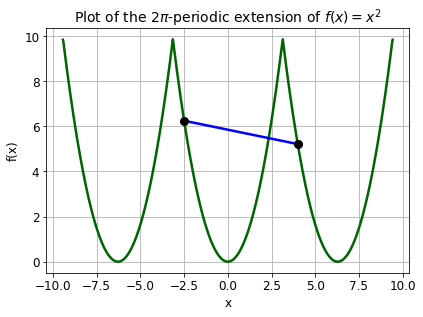
\includegraphics[width=\textwidth]{Pictures/Periodic_function_NC.png}
    \caption{2D plot of $f$}\label{fig:periodic_f}
  \end{minipage}
  \hspace{0.3cm} 
  \begin{minipage}[b]{0.37\textwidth}
    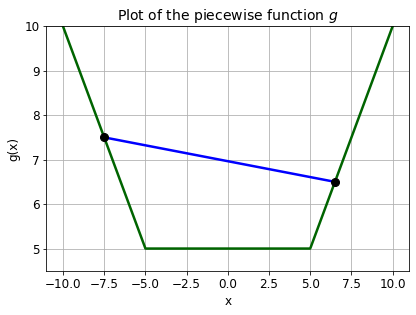
\includegraphics[width=\textwidth]{Pictures/piecewise_function_C.png}
    \caption{2D plot of $g$}\label{fig:piecewise_g}
  \end{minipage}
\end{figure}\\
The function depicted in Figure \ref{fig:periodic_f} is non-convex, because it does not satisfy the inequality given in Equation \eqref{eq:3}. This can be observed from the plot, where the line segment connecting two function values intersects the graph of the function at a point that is not one of the endpoints of the line segment. In contrast, the function shown in Figure \ref{fig:piecewise_g} is convex, because it is not possible to draw a line segment between any two function values in a way that intersects the graph of the function at a point other than the endpoints. As a result, this function satisfies Equation \eqref{eq:3}.
In the field of optimization, we frequently encounter multi-dimensional functions. These are functions with $\textbf{dom} (f)=\mathbb{R}^{n},$ where $n\in\mathbb{N}$ and $n > 1$. We consider two examples on $\mathbb{R}^2$, starting with a convex quadratic function, $f$:
\begin{equation*}\label{eq:10}\tag{2.5}
\begin{aligned}
&f(x) = \frac{1}{2}(x_{1}^{2} + 10x_{2}^{2})
\end{aligned}
\end{equation*}
Now, we compare this with a non-convex function, which we'll denote as $g$:
\begin{equation*}\label{eq:11}\tag{2.6}
\begin{aligned}
&g(x) = \frac{\sin\left(0.5x_1^2 - 0.25x_2^2 + 3\right)}{0.5 + 0.25x_1^2 + x_2^2}
\end{aligned}
\end{equation*}
Figures \ref{fig:ellipsoid_3D} and \ref{fig:Nonconvex_3D} are 3D plots of these functions.\footnote{Refer to Notebook 6, cells 4 and 5, in GitHub \cite{ThesisCode2023} for the code to create the plots.}
\begin{figure}[h]
  \centering
  \begin{minipage}[b]{0.38\textwidth}
    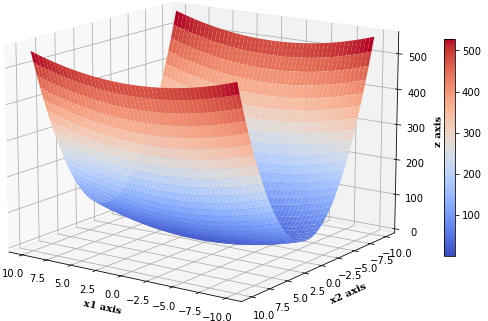
\includegraphics[width=\textwidth]{Pictures/3D plot of ellipsoid.png}
    \caption{3D plot of $f$}\label{fig:ellipsoid_3D}
  \end{minipage}
  \hspace{0.3cm} 
  \begin{minipage}[b]{0.38\textwidth}
    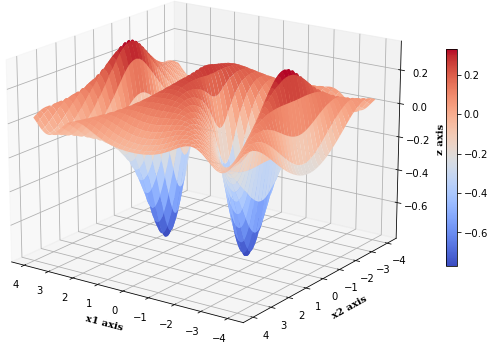
\includegraphics[width=\textwidth]{Pictures/3D plot of non convex.png}
    \caption{3D plot of $g$}\label{fig:Nonconvex_3D}
  \end{minipage}
\end{figure}\\
Visually, $f$ in Figure \ref{fig:ellipsoid_3D} represents an elliptical bowl and its graph has a parabolic shape. Clearly the optimal solution is $x^{*} = (0,0)$ with $f(x^{*}) = 0$. By visual inspection of the graph of $g$ in Figure \ref{fig:Nonconvex_3D}, one can easily verify that $g$ is non-convex, since it has many local minima and maxima. Such exploration of function properties isn't just theoretical, it has practical applications in fields like machine learning. In this domain, optimization techniques are used to train models to effectively carry out tasks. 
\newpage
In this setting, the objective function $f_0$ represents a cost function that measures the difference between the model's predictions and the true target values. The optimization problem is then to find the parameters of the model that minimize this cost function, subject to any constraints specified by the constraint functions $f_i$ and bounds $b_i$. In deep learning (a subset of machine learning), the model of choice is typically a neural network. A neural network is a computational model inspired by the human brain's own network of neurons. It consists of interconnected layers of nodes, or "neurons", and each connection has an associated weight that gets adjusted during the learning process. In the context of optimizing a cost function $f_0$, the variable $x$ represents the weights and biases of the network. The optimization problem, therefore, is to determine the values of these weights and biases that result in the best performance for a given task. This performance is evaluated using a cost function, a measure of how well the model is doing. The importance of optimization in machine learning and deep learning lies in its ability to train models that can generalize well to new data and perform well on the desired task. The optimization problem provides a framework for finding the best possible parameters of the model, given the cost function and any constraints, and is a crucial step in the training process for machine learning and deep learning models. Usually, the cost function is either convex or non-convex. Convex optimization problems can often be solved efficiently using well-established optimization algorithms, such as Deterministic Gradient Descent, often called Batch Gradient Descent (BGD). This algorithm can converge relatively quickly to a global minimum, but the convergence rate can depend on various factors, such as the dimensionality of the problem. Unfortunately, most cost functions encountered in machine learning are non-convex and high dimensional, making it hard to locate a global minimum. Luckily, it's not all bad news. In non-convex optimization, BGD has the capacity to locate at least a local minimum. In practice, such a solution is often considered satisfactory. A second challenge encountered in non-convex optimization is that the dimensionality of the problem is often very high. This makes BGD an unfavourable choice for solving the optimization as BGD requires the computation of the full gradient at every step of the algorithm. In this setting, a different class of algorithms, known as stochastic optimization algorithms, can be employed. One of these, is the famous Stochastic Gradient Descent (SGD). The key difference between between SGD and BGD, lies in their handling of high dimensionality. SGD manages this issue by computing stochastic estimates of the full gradient of the cost function during each step of the algorithm. A second advantage of SGD over BGD is its inherent stochasticity, which enables the algorithm to escape 'bad' local minima. This is a significant advantage over BGD, which can get trapped in a local minimum once it reaches one. One thing that SGD and BGD have in common, is that both are gradient-based optimization algorithms. In other words, they operate under the assumption that the cost function is differentiable. This may seem restrictive, as not all functions possess this property. Fortunately, there exists a class of optimization algorithms that aren't bound by this assumption: stochastic global optimization algorithms. These methods are especially valuable in tackling non-convex optimization problems. By employing various search strategies, they can explore the solution space more thoroughly, thereby increasing the odds of identifying the global minimum. Two such algorithms stand out: Simulated Annealing (SA) and Particle Swarm Optimization (PSO). SA is inspired by the process of annealing in metallurgy, where it's used to alter the physical properties of a material. The algorithm gradually cools the system over time, altering the solution space to help escape local minima and reach a global minimum. On the other hand, PSO draws inspiration from the social behavior of bird flocking or fish schooling. It involves a group of candidate solutions, called 'particles', moving through the solution space. Each particle adjusts its path based on its own experience and that of neighboring particles. This collective behavior helps explore the solution space more thoroughly, improving the chance of finding a global minimum. The topics introduced here will be discussed in greater detail and various applications of these topics will be showcased in this thesis.\footnote{Refer to Notebooks 1-7 on GitHub \cite{ThesisCode2023} for the implementation of the applications discussed in this thesis.}





















